%%%%%%%%%%%%%%%%%%%%%%%%%%%%%%%%%%%%%%%%%%%%%%%%%%%%%%%%%%%%%%%%%%%%%%%%%%%%%%%%
%2345678901234567890123456789012345678901234567890123456789012345678901234567890
%        1         2         3         4         5         6         7         8
% THESIS CHAPTER

\chapter{Work Undertaken}

% short summary of the chapter
\section*{Measures}

\section*{Summary}
short summary of the chapter.

\section{Labelled UI and Explanation}
Blah, pictures, talk about some high level decisions and poit out key parts.

\section{Solving the problem}
Blah, pictures, talk about some high level decisions and poit out key parts.

\section{Network Choice}
Networks vary enormously. There are applications from communications to city planning and counter terrorism to the nervous system.[source] Solving the Dynamic Network interpretation problem could feasibly be done on any type of network. For the purposes of this report, a social network was used. Social networks are readily understood and require virtually no domain knowledge, compared with say, biological networks.[source] Since this project aims to tackle dynamic network interpretation, using a simple network as a baseline ensures that difficulties in comprehension aren’t just inherent to the domain but the network itself. Social networks also tend to be comparatively small. (The largest social network is probably facebook so 1-2 billion nodes?)[source]. The network used is small. There are also a variety of existing networks that could be used to test against.

Social network analysis provides a novel window by allowing the impacts to be quantified at the individual level, and the links between past, current and future behaviour to be carried across contexts. <https://besjournals.onlinelibrary.wiley.com/doi/pdf/10.1111/1365-2656.12764>


\section{The Databar}

\begin{center}
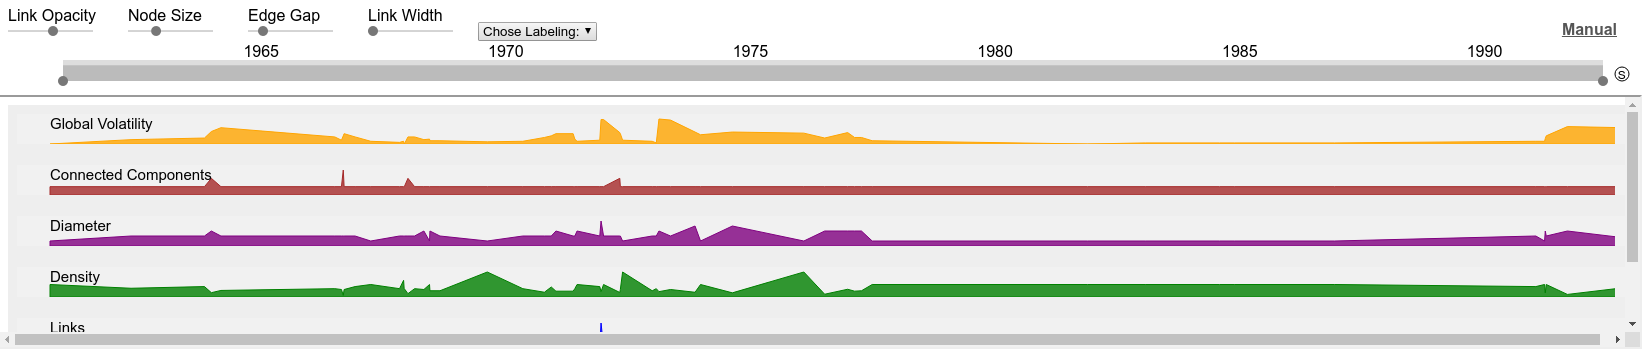
\includegraphics[trim={0 0 0 0}, width=140mm]{./Figures/databar.png}
\end{center}

The Databar holds the global visualisation graphs. I decided to place it along the top of the window because it would line up nicely with the pre-existing timeline which could then double as the x-axis label - saving valuable screen space.
The databar is highly interactive. Each graph is initially collapsed and can then be expanded by clicking.
\begin{center}
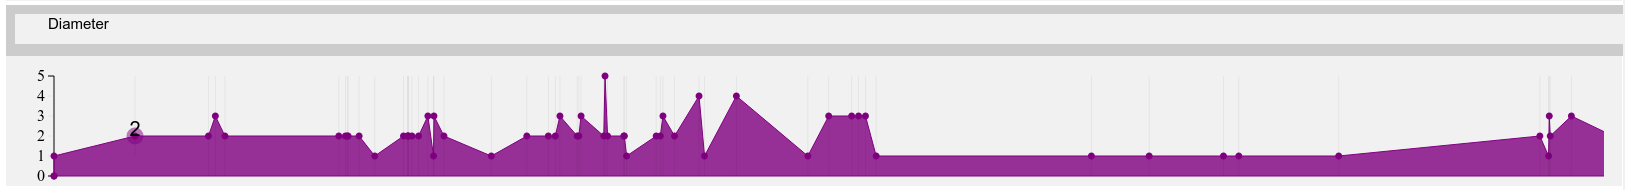
\includegraphics[trim={0 0 0 0}, width=140mm]{./Figures/diameterGraph.png}
\end{center}
Moving the mouse across the screen causes a cursor to track along the ridgeline of the graph. the y-label at that point is shown on the tracker.
\begin{center}
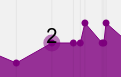
\includegraphics[trim={0 0 0 0}, width=35mm]{./Figures/ridgeTracker.png}
\end{center}
The vertical lines indicate a timestep/change in the graph. This can be useful for comparing graphs vertically and for easily finding time periods of high or low activity.
Finally, graphs can be reordered for easy comparison using click and drag.

\section{Measures and Visualisations}


%%%%%%%%%%%%%%%%%%%%%%%%%%%%%%%%%%%%%%%%%%%%%%%%%%%%%%%%%%%%%%%%%%%%%%%%%%%%%%%%%%%%%%%%%%%%%%%%%%%%%%%%%%%%%%%
%VOLATILITY
%%%%%%%%%%%%%%%%%%%%%%%%%%%%%%%%%%%%%%%%%%%%%%%%%%%%%%%%%%%%%%%%%%%%%%%%%%%%%%%%%%%%%%%%%%%%%%%%%%%%%%%%%%%%%%%

\subsection{Volatility}

\subsubsection{Development}
In my literature review I didn’t come across any examples where this specific measure was used or investigated. I felt that there needed to be some measure or score which captured the level of node connection fluctuation such that a node whose connections tended to stay mostly within a fixed set of other nodes would score low but a node whose edges tended to be short lived and with unfamiliar nodes would score high.
Volatility is a local measure and is calculated with respect to a set start time and end time. Initially it was calculated as the population standard deviation of the number of a node’s connections throughout that time period, effectively the variance in the number of connections.

\begin{center}
population standard deviation = $\sqrt{\frac{1}{N} \sum_{i=1}^N (x_i - \overline{x})^2}$
\end{center}

Examples are given below.


\begin{center}
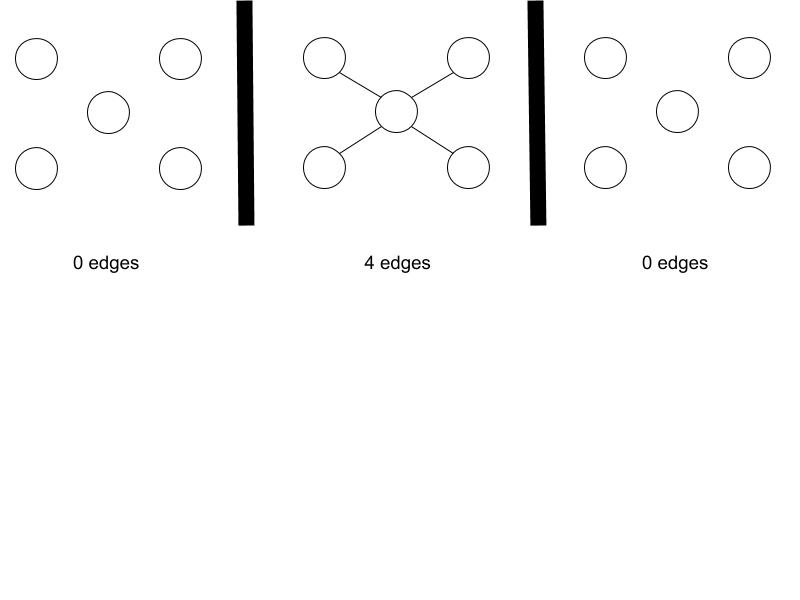
\includegraphics[trim={0 10cm 0 -1cm}, width=120mm]{./Figures/volatility1.jpg}

$N = 3$

$\overline{x} = \frac{4 + 0 + 0}{3} = \frac{4}{3}$

$volatility =\frac{1}{3}\times((0 - \frac{4}{3})^2 + ((4 - \frac{4}{3})^2) + (0 - \frac{4}{3})^2) $

$volatility = 1.89$

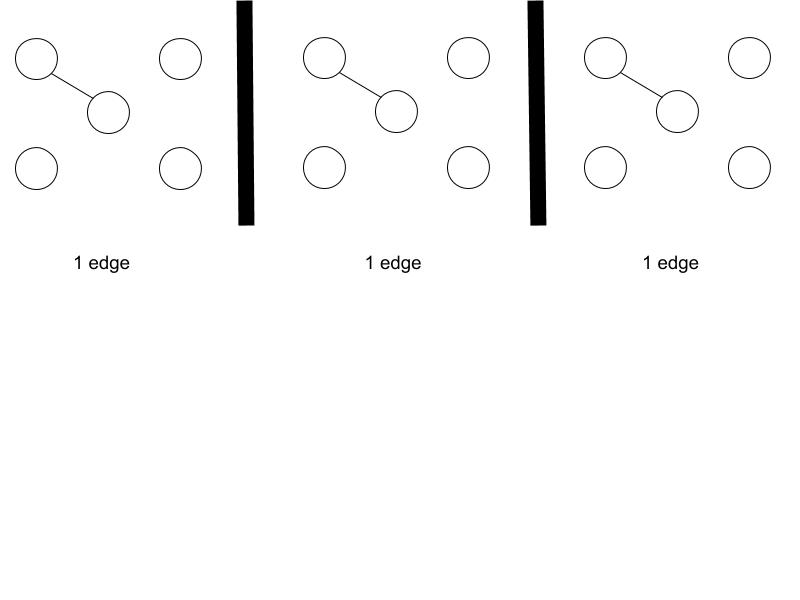
\includegraphics[trim={0 10cm 0 -1cm}, width=120mm]{./Figures/volatility2.jpg}

$N = 3$

$\overline{x} = \frac{1 + 1 + 1}{3} = 1$

$volatility =\frac{1}{3}((1 - 1)^2 + ((1 - 1)^2) + (1 - 1)^2) $

$volatility = 0$
\end{center}

This approach appeared to work quite well - changes in edges results in a higher volatility whereas no changes results in 0 volatility.

However the problem with this approach is that it maintains no ‘memory’ of which edges were previously connected, consider the example below.
\begin{center}
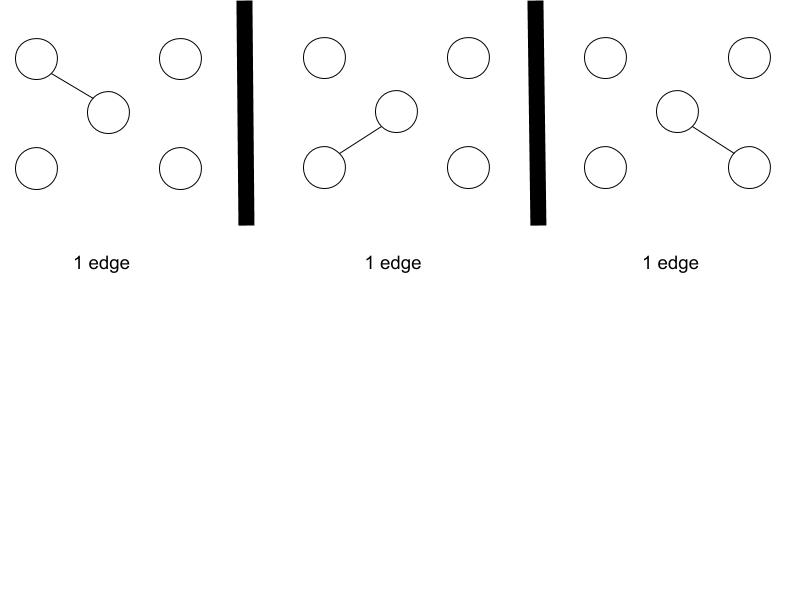
\includegraphics[trim={0 10cm 0 -1cm}, width=120mm]{./Figures/volatility3.jpg}
\end{center}

The volatility will still be 0 despite the edge changing since only the number of edges is taken into account.
To fix this we give edges unique ids and store a binary value tracking which edges are present at each time frame and then sum the standard deviations of these. Example below <I THINK THIS IS INCORRECT AND 2 SHOULDN'T BE THERE:

\begin{center}
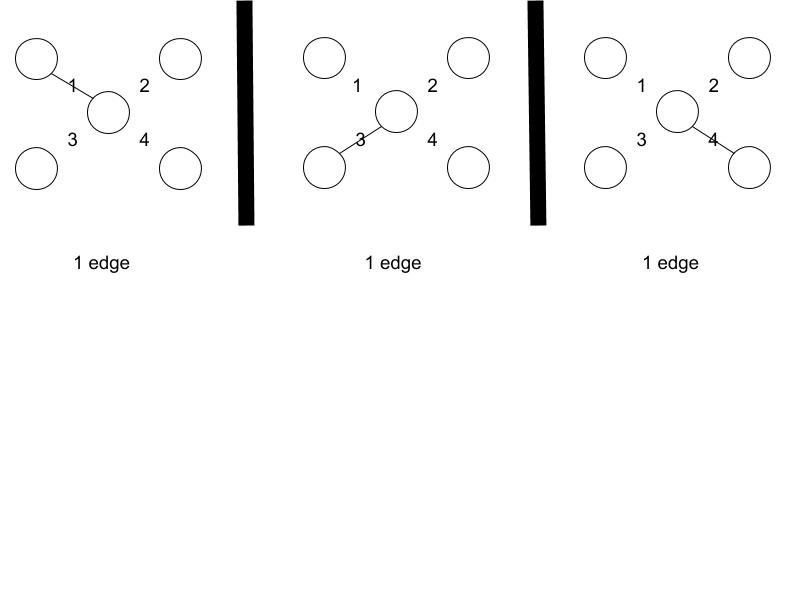
\includegraphics[trim={0 10cm 0 -1cm}, width=120mm]{./Figures/volatility4.jpg}
\end{center}

We store an object mapping edge:[binary value indicating presence during timestep at index].
\begin{center}
\{1:[1, 0, 0], 2: [0, 0, 0], 3: [0, 1, 0], 4: [0, 0, 1]\}
\end{center}
We then calculate volatility as the average of the standard deviations of the object values.
\begin{center}
$volatility = \frac{std([1,0,0]) + std([0,0,0]) + std([0,1,0]) + std([0,0,1])}{4}$

$volatility = 0.35$
\end{center}

<Something about why that data structure makes sense despite the rather large space complexity, it doesn't quite - you could just keep a counter for each edge so if counter was 4 and timesteps were 5 you would do std([1,1,1,1,0]) which would be esay to code - or could be further optimised?, ask BB about this.>

\subsubsection{Vistorian Implementation}
Whilst this solution would work well in a general case it unfortunately works poorly in The Vistorian as edges only appear once. To fix this we instead use node-pairs. 
Volatility in The Vistorian indicates the variance in the number of letters sent and received by a node in a given period. This is useful in the Vistorian because it allows us to see if one contact was rapidly sending or receiving messages to or from new contacts, or if they maintained fairly constant communication with a select number. 

\subsubsection{Visualisation Method}
For visualisation ‘spikes’ are used, where more spikes indicates higher volatility. Other methods were considered, vibration matches with the mental image of volatility but would be too distracting to the eye. Dotted rings with larger diameter indicating higher volatility were considered but had too much potential for confusing overlap. Colours were originally used but could be misconstrued as relating to the edge colours. 

\subsubsection{Further Applications}
Volatility could have broad applications in other domains where dynamic networks are used. 
\newline\newline
Say a system administrator was conducting a post-mortem of an attack on a network using a dynamic network analysis tool to determine which nodes were potentially behaving maliciously. One measure useful in determining an anomaly in a network is the number of successfully established TCP connections in a time interval \cite{fnpfid}. A malicious port scan usually sends a relatively small number of packets to a large number of hosts on a network \cite{fnpfid}. If a similar volatility measure was implemented in this dynamic network analysis tool and TCP connections were considered to be edges it would be very easy for the system administrator to spot particularly volatile, or spiky, nodes.
\newline\newline
Whilst investigating different proteins in protein-protein interaction networks and their impact on the development and progression of hepatocellular carcinoma (HCC) after hepatitis C virus infection the protein core ESR1, which interacted with most of the nodes in the randomly selected sub-network, was shown to be associated with an increased HCC risk \cite{acaotdbnihih}. Using volatility as a measure while performing this anaylsis would have immediately highlighted the ESR1 protein as highly volatile and worthy of further investigation.

%%%%%%%%%%%%%%%%%%%%%%%%%%%%%%%%%%%%%%%%%%%%%%%%%%%%%%%%%%%%%%%%%%%%%%%%%%%%%%%%%%%%%%%%%%%%%%%%%%%%%%%%%%%%%%%
%NUMBER OF LINKS
%%%%%%%%%%%%%%%%%%%%%%%%%%%%%%%%%%%%%%%%%%%%%%%%%%%%%%%%%%%%%%%%%%%%%%%%%%%%%%%%%%%%%%%%%%%%%%%%%%%%%%%%%%%%%%%
\subsection{Number of links}
\subsubsection{Summary}
Simply the number of edges. This gives a quick idea of the degree of activity during a time frame. 

\subsubsection{Reasons for Selection}
The number of edges is one of the most basic measures. However it aids understanding of the network considerably as it provides perhaps the simplest way of understanding the overall activity of the network, keeping cognitive load low while still improving understanding considerably.

\subsubsection{Vistorian Implementation}
This is useful in the Vistorian because the number of messages sent in each given time frame can quickly be seen.
\subsubsection{Visualisation}
\subsubsection{Further Applications}


%%%%%%%%%%%%%%%%%%%%%%%%%%%%%%%%%%%%%%%%%%%%%%%%%%%%%%%%%%%%%%%%%%%%%%%%%%%%%%%%%%%%%%%%%%%%%%%%%%%%%%%%%%%%%%%
%NUMBER OF CONNECTED NODES
%%%%%%%%%%%%%%%%%%%%%%%%%%%%%%%%%%%%%%%%%%%%%%%%%%%%%%%%%%%%%%%%%%%%%%%%%%%%%%%%%%%%%%%%%%%%%%%%%%%%%%%%%%%%%%%
\subsection{Number of connected nodes}
\subsubsection{Summary}
The number of nodes with at least one edge in the given period.

\subsubsection{Reasons for Selection}
Like the number of edges, the number of connected nodes is also a very basic measure. However it gives an easily interpretable sense of the number of actors at a given time. Knowing if activity is high because there are multiple actors or because those actors are each very active is important to be able to distinguish. As it is a simple measure it also keeps cognitive load low while still improving understanding considerably.

\subsubsection{Vistorian Implementation}
In the Vistorian this gives an idea of the number of people involved at each time frame. 

\subsubsection{Visualisation}
\subsubsection{Further Applications}

%%%%%%%%%%%%%%%%%%%%%%%%%%%%%%%%%%%%%%%%%%%%%%%%%%%%%%%%%%%%%%%%%%%%%%%%%%%%%%%%%%%%%%%%%%%%%%%%%%%%%%%%%%%%%%%
%DIAMETER
%%%%%%%%%%%%%%%%%%%%%%%%%%%%%%%%%%%%%%%%%%%%%%%%%%%%%%%%%%%%%%%%%%%%%%%%%%%%%%%%%%%%%%%%%%%%%%%%%%%%%%%%%%%%%%%
\subsection{Diameter}
\subsubsection{Summary}
The longest of all shortest paths in the network. This was implemented using [HOW I DID IT/algorithm] Diameter gives a sense of the interconnectedness of a network.

\subsubsection{Reasons for Selection}
Diameter is particularly important in social networks. The commonly known six-degrees of separation theory https://www.jstor.org/stable/pdf/2786545.pdf?acceptTC=true effectively states that if one were to make a social networks of all humans, the expected diameter would be 6. In a dynamic context... 

\subsubsection{Vistorian Implementation}
In The Vistorian the diameter gives a sense of social distance or degrees of separation between individuals in a ‘conversation’. <may need defined> 
\subsubsection{Visualisation}
\subsubsection{Further Applications}

%%%%%%%%%%%%%%%%%%%%%%%%%%%%%%%%%%%%%%%%%%%%%%%%%%%%%%%%%%%%%%%%%%%%%%%%%%%%%%%%%%%%%%%%%%%%%%%%%%%%%%%%%%%%%%%
%DENSITY
%%%%%%%%%%%%%%%%%%%%%%%%%%%%%%%%%%%%%%%%%%%%%%%%%%%%%%%%%%%%%%%%%%%%%%%%%%%%%%%%%%%%%%%%%%%%%%%%%%%%%%%%%%%%%%%
\subsection{Density}
\subsubsection{Summary}
Density here is defined as (THIS FORMULA). It gives a sense of connectedness at a given period of time. Only nodes with at least one edge are counted. Essentially, if every node is connected to every other node then density will be 1. 

\subsubsection{Reasons for Selection}
Density is used as one of the 7 measures because it gives the user an overview of how interconnected the graph is at a given point and how that varies over time. Since the goal is to provide as much information about the behaviour of the graph as possible using as few measures as possible it is important that information overlap from different measures is minimised. An overview of density can't be easily gathered from observing the graph and it can't be easily extrapolated from the other selected methods.

\subsubsection{Vistorian Implementation}
We define an active node as node that has sent or received a letter during a time frame. In The Vistorian a density of 1 at a time frame means that every  active node during that time frame has either sent or received a letter from every other active node.

\subsubsection{Visualisation}
Density is visualised in the DataBar along with the other global methods. This is detailed in <a>.

\subsubsection{Further Applications}
<a>.

%%%%%%%%%%%%%%%%%%%%%%%%%%%%%%%%%%%%%%%%%%%%%%%%%%%%%%%%%%%%%%%%%%%%%%%%%%%%%%%%%%%%%%%%%%%%%%%%%%%%%%%%%%%%%%%
%NUMBER OF CONNECTED COMPONENTS
%%%%%%%%%%%%%%%%%%%%%%%%%%%%%%%%%%%%%%%%%%%%%%%%%%%%%%%%%%%%%%%%%%%%%%%%%%%%%%%%%%%%%%%%%%%%%%%%%%%%%%%%%%%%%%%
\subsection{Number of connected components}
\subsubsection{Summary}
A connected component is a full group of nodes connected by edges. This measure is simply the number of discrete connected components.
Figure below has two connected components.

\begin{center}
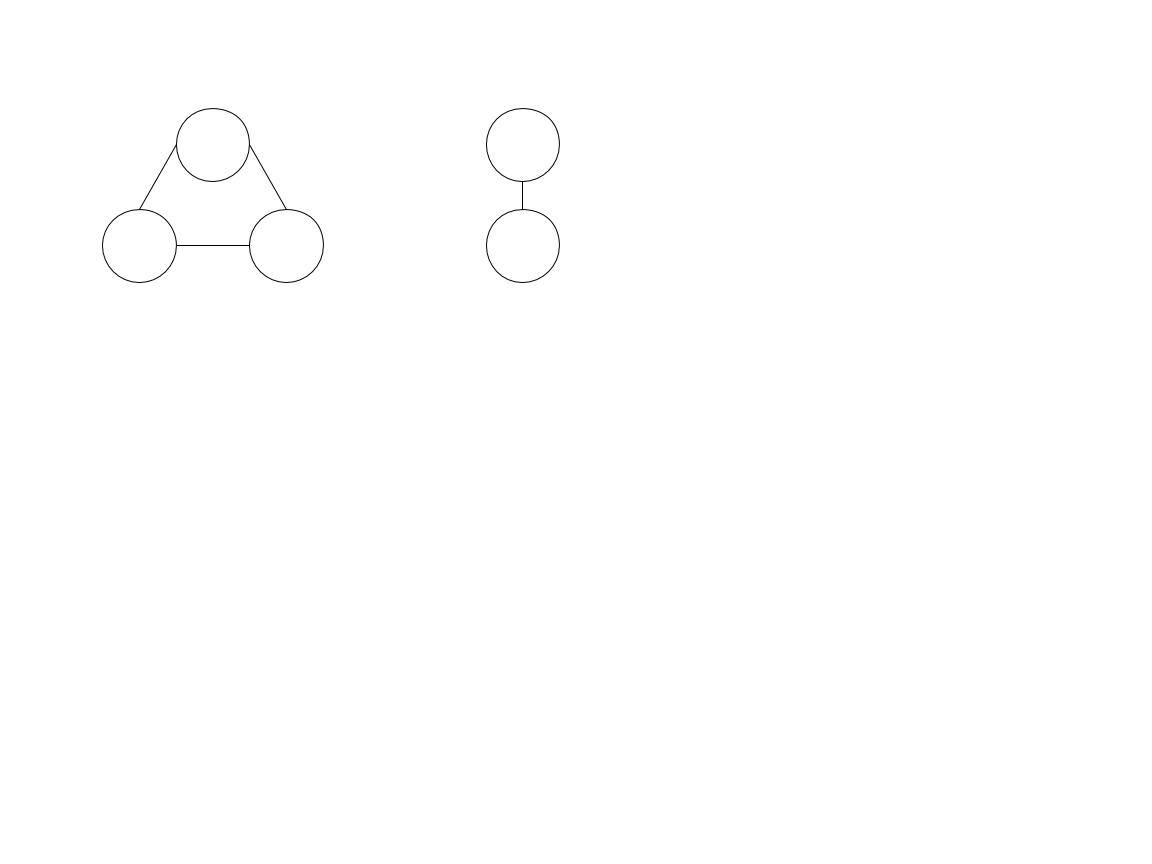
\includegraphics[trim={0cm, 20cm, -10cm, 0cm}, width=180mm]{./Figures/connectedComponents1.jpg}
\end{center}

\subsubsection{Reasons for Selection}
\subsubsection{Vistorian Implementation}
In The Vistorian, this measure can be interpreted as the number of distinct conversations happening during a given chunk of time. 
Should I provide details of the algorithm?

\subsubsection{Visualisation}
\subsubsection{Further Applications}

%%%%%%%%%%%%%%%%%%%%%%%%%%%%%%%%%%%%%%%%%%%%%%%%%%%%%%%%%%%%%%%%%%%%%%%%%%%%%%%%%%%%%%%%%%%%%%%%%%%%%%%%%%%%%%%
%CENTRALITY
%%%%%%%%%%%%%%%%%%%%%%%%%%%%%%%%%%%%%%%%%%%%%%%%%%%%%%%%%%%%%%%%%%%%%%%%%%%%%%%%%%%%%%%%%%%%%%%%%%%%%%%%%%%%%%%
\subsection{Centrality}
\subsubsection{Summary}
Centrality is a local measure. The specific implementation used is betweenness centrality. 

\subsubsection{Reasons for Selection}

\subsubsection{Vistorian Implementation}
Centrality is 

\subsubsection{Visualisation}
\subsubsection{Further Applications}

